\section{Asset Pricing: Lucas Tree and Complete Markets}

This section has two parts. Part one is the Lucas (1978) tree model: a single representative household prices a risky asset (a ``tree''), and we derive the consumption-based asset-pricing formula. Part two is the complete-markets (Arrow--Debreu) economy with many households: we derive the equilibrium allocation, show that it coincides with a planner's solution, and use Arrow--Debreu prices to price any asset.

%======================================================================
\subsection{Lucas tree model: setup \pg{18}}

\paragraph{Setup.}
\begin{itemize}
  \item \textbf{Time} is discrete, $t=0,1,2,\dots$; agents live forever and discount the future with factor $\beta\in(0,1)$.
  \item \textbf{Assets.} The only assets are identical, infinitely lived \emph{trees}. Each tree yields $d_t$ units of fruit in period $t$. $d_t$ is random and exogenous (the ``dividend''). Fruit is \emph{nondurable}: it must be eaten in the period it appears or it rots.
  \item \textbf{Endowment economy}: there is no production and no storage. The only goods available are the fruit.
  \item \textbf{Notation.}
  \begin{itemize}
    \item $C_t$: consumption of fruit per person; $L_t$: population.
    \item $k_t$: number of trees (shares) per person; $k^i_t$: trees held by household $i$ at the \emph{start} of period $t$.
    \item $p_t$: equilibrium price of one tree, in units of fruit. It is an \emph{ex-dividend} price: if a tree is sold in period $t$, the sale happens \emph{after} the current owner has collected the fruit $d_t$.
    \item $u(\cdot)$: period utility, with $u'>0$, $u''<0$.
    \item $E_t[\cdot]$: expectation conditional on all information available at date $t$ (in particular $d_t$ and $p_t$ are known at $t$).
  \end{itemize}
  \item \textbf{Resource constraint}: aggregate consumption equals aggregate fruit,
  \begin{equation}\label{eq:s4_rc}
    C_tL_t = d_t k_t L_t \quad\Longleftrightarrow\quad C_t = d_t k_t .
  \end{equation}
  Normalizing the supply of trees to one per person ($k_t=1$) gives $C_t=d_t$.
\end{itemize}

\paragraph{Household budget constraint.}
In period $t$ household $i$ arrives with $k^i_t$ trees. Its income is the fruit from those trees plus the value of the trees if sold. It spends on consumption and on the trees it carries into $t+1$:
\begin{equation}\label{eq:s4_bc}
  \underbrace{p_t k^i_{t+1} + C^i_t}_{\text{spending: new trees + consumption}}
  \;=\;
  \underbrace{(d_t + p_t)\,k^i_t}_{\text{income: dividends + value of trees}} .
\end{equation}
Solve \eqref{eq:s4_bc} for next period's holdings. Subtract $C^i_t$ and divide by $p_t$:
\begin{align}
  k^i_{t+1} &= \frac{(d_t+p_t)k^i_t - C^i_t}{p_t} \notag\\
            &= \Big(1+\frac{d_t}{p_t}\Big)k^i_t - \frac{C^i_t}{p_t}. \label{eq:s4_lom_k}
\end{align}

\paragraph{Wealth and return.}
Define wealth at the start of $t$ (value of fruit plus value of trees) and the gross return on a tree from $t$ to $t+1$:
\begin{equation}\label{eq:s4_def_mR}
  m^i_t \equiv (p_t+d_t)\,k^i_t,
  \qquad
  R_{t+1} \equiv \frac{p_{t+1}+d_{t+1}}{p_t}.
\end{equation}
$R_{t+1}$ = (capital gain + dividend) per unit of money invested. Derive the law of motion of wealth:
\begin{align}
  m^i_{t+1} &= (p_{t+1}+d_{t+1})\,k^i_{t+1} && \text{(definition at $t+1$)}\notag\\
  &= (p_{t+1}+d_{t+1})\,\frac{(d_t+p_t)k^i_t - C^i_t}{p_t} && \text{(substitute \eqref{eq:s4_lom_k})}\notag\\
  &= \frac{p_{t+1}+d_{t+1}}{p_t}\,\big(m^i_t - C^i_t\big) && \text{(use $m^i_t=(p_t+d_t)k^i_t$)}\notag\\
  &= R_{t+1}\,\big(m^i_t - C^i_t\big). && \text{(definition of $R_{t+1}$)} \label{eq:s4_lom_m}
\end{align}
Interpretation: whatever wealth is not eaten is invested in trees and earns the random gross return $R_{t+1}$.

\paragraph{Household problem.}
The household chooses a consumption plan to maximize expected discounted utility from date $t$ onward (expectations are taken at $t$, not at $0$):
\begin{equation}\label{eq:s4_seq}
  V(m^i_t) = \max_{\{C^i_{t+n}\}_{n\ge0}} E_t\sum_{n=0}^{\infty}\beta^n u(C^i_{t+n})
  \quad\text{s.t. \eqref{eq:s4_lom_m} in every period.}
\end{equation}
The value function $V$ depends on current wealth $m^i_t$ (it also depends on the current state of the dividend process, which we suppress). The recursive (Bellman) form is
\begin{equation}\label{eq:s4_bellman}
  V(m^i_t) = \max_{C^i_t}\Big\{u(C^i_t) + \beta E_t\big[V(m^i_{t+1})\big]\Big\},
  \qquad m^i_{t+1} = R_{t+1}(m^i_t - C^i_t).
\end{equation}
We substitute the law of motion for $m^i_{t+1}$ directly into the objective, so there is no separate constraint or multiplier.

%======================================================================
\subsection{Euler equation and the stochastic discount factor \pg{18--19}}

\paragraph{Step 1: first-order condition.}
Differentiate the right-hand side of \eqref{eq:s4_bellman} with respect to $C^i_t$ (chain rule: $\frac{d}{dC}V(m(C)) = V'(m)\,\frac{\partial m}{\partial C}$):
\begin{align*}
  0 &= u'(C^i_t) + \beta E_t\Big[V'(m^i_{t+1})\,\frac{\partial m^i_{t+1}}{\partial C^i_t}\Big].
\end{align*}
From \eqref{eq:s4_lom_m}, $\partial m^i_{t+1}/\partial C^i_t = -R_{t+1}$. Substitute and move the expectation term to the left:
\begin{equation}\label{eq:s4_foc}
  u'(C^i_t) = \beta E_t\big[R_{t+1}\,V'(m^i_{t+1})\big].
\end{equation}
Meaning: eating one more unit today gives $u'(C^i_t)$; investing it instead gives $R_{t+1}$ units of wealth tomorrow, each worth $V'(m^i_{t+1})$, discounted by $\beta$.

\paragraph{Step 2: envelope condition.}
\emph{Envelope theorem}: if $V(\theta)=\max_x f(x,\theta)$ with maximizer $x^*(\theta)$, then $V'(\theta) = \partial f(x^*,\theta)/\partial\theta$ (the indirect effect through $x^*$ is zero because $\partial f/\partial x=0$ at the optimum).
Apply it to \eqref{eq:s4_bellman} with $\theta = m^i_t$. Since $\partial m^i_{t+1}/\partial m^i_t = R_{t+1}$,
\begin{align*}
  V'(m^i_t) &= \beta E_t\big[R_{t+1}\,V'(m^i_{t+1})\big] && \text{(envelope theorem)}\\
            &= u'(C^i_t). && \text{(by the FOC \eqref{eq:s4_foc})}
\end{align*}
This holds at every date, so shifting it one period forward:
\begin{equation}\label{eq:s4_env}
  V'(m^i_{t+1}) = u'(C^i_{t+1}).
\end{equation}
The marginal value of wealth equals the marginal utility of consumption.

\paragraph{Step 3: Euler equation.}
Substitute \eqref{eq:s4_env} into \eqref{eq:s4_foc}, then the definition of $R_{t+1}$:
\begin{align*}
  u'(C^i_t) &= \beta E_t\big[R_{t+1}\,u'(C^i_{t+1})\big]\\
  &= \beta E_t\Big[\frac{p_{t+1}+d_{t+1}}{p_t}\,u'(C^i_{t+1})\Big].
\end{align*}
Multiply both sides by $p_t$ and divide by $u'(C^i_t)$ (both are known at $t$, so they can move inside $E_t$):
\begin{equation}\label{eq:s4_euler_i}
  p_t = \beta E_t\!\left[\frac{u'(C^i_{t+1})}{u'(C^i_t)}\,(p_{t+1}+d_{t+1})\right].
\end{equation}
This is the asset-pricing Euler equation, a \emph{first-order stochastic difference equation} in $p_t$. Interpretation: at the optimum the cost of a tree today ($p_t$, in fruit) equals the expected value of what it pays tomorrow (price + dividend), converted into today's fruit using the marginal rate of substitution $\beta u'(C_{t+1})/u'(C_t)$.

\paragraph{Step 4: equilibrium.}
All households are identical (representative agent), and fruit cannot be stored. So in equilibrium everybody holds one tree and eats its fruit: $C^i_t = C_t = d_t$ (from \eqref{eq:s4_rc} with $k_t=1$). The only source of goods is $d$, and what comes in must be eaten. Substituting $C_t=d_t$ into \eqref{eq:s4_euler_i}:

\begin{keybox}[title=Lucas asset-pricing formula]
\begin{equation}\label{eq:s4_lucas}
  p_t = \beta E_t\!\left[\frac{u'(d_{t+1})}{u'(d_t)}\,(p_{t+1}+d_{t+1})\right]
  \quad\Longleftrightarrow\quad
  p_t = E_t\big[M_{t,t+1}\,(p_{t+1}+d_{t+1})\big],
\end{equation}
where the \textbf{stochastic discount factor (SDF)} between $t$ and $t+n$ is
\begin{equation}\label{eq:s4_sdf}
  M_{t,t+n} \equiv \beta^n\,\frac{u'(d_{t+n})}{u'(d_t)} .
\end{equation}
Dividing \eqref{eq:s4_lucas} by $p_t$ gives the equivalent form $1 = E_t\big[M_{t,t+1}R_{t+1}\big]$.
\end{keybox}
The SDF is ``stochastic'' because $d_{t+n}$ is random: a unit of fruit at $t+n$ is worth more today if it arrives in a state where fruit is scarce ($d_{t+n}$ low, $u'(d_{t+n})$ high). Note $M_{t,t+1}M_{t+1,t+2}=M_{t,t+2}$: the $u'(d_{t+1})$ terms cancel.

\paragraph{Risk-free rate.} A one-period risk-free bond pays $1$ for sure at $t+1$. Applying \eqref{eq:s4_lucas} to its payoff (price $=E_t[M_{t,t+1}\cdot 1]$) gives the gross risk-free rate $1+r_{f,t} = 1/E_t[M_{t,t+1}]$.

%======================================================================
\subsection{Iterating forward: price = present value of dividends \pg{19}}

Equation \eqref{eq:s4_lucas} links $p_t$ to $p_{t+1}$. Iterating it removes future prices.

\emph{Law of iterated expectations}: $E_t\big[E_{t+1}[X]\big]=E_t[X]$.

Write \eqref{eq:s4_lucas} at $t+1$: $p_{t+1}=E_{t+1}[M_{t+1,t+2}(p_{t+2}+d_{t+2})]$. Substitute into \eqref{eq:s4_lucas} at $t$:
\begin{align*}
  p_t &= E_t\big[M_{t,t+1}d_{t+1}\big] + E_t\big[M_{t,t+1}\,p_{t+1}\big]\\
  &= E_t\big[M_{t,t+1}d_{t+1}\big] + E_t\Big[M_{t,t+1}\,E_{t+1}\big[M_{t+1,t+2}(p_{t+2}+d_{t+2})\big]\Big]
     && \text{(substitute $p_{t+1}$)}\\
  &= E_t\big[M_{t,t+1}d_{t+1}\big] + E_t\big[M_{t,t+2}(p_{t+2}+d_{t+2})\big]
     && \text{(iterated exp.; $M_{t,t+1}M_{t+1,t+2}=M_{t,t+2}$)}\\
  &= E_t\big[M_{t,t+1}d_{t+1}+M_{t,t+2}d_{t+2}\big] + E_t\big[M_{t,t+2}\,p_{t+2}\big].
\end{align*}
Repeating $n$ times:
\begin{equation}\label{eq:s4_iter}
  p_t = E_t\sum_{j=1}^{n} M_{t,t+j}\,d_{t+j} \;+\; E_t\big[M_{t,t+n}\,p_{t+n}\big].
\end{equation}
\textbf{No-bubble (transversality) condition}: $\lim_{n\to\infty}E_t[M_{t,t+n}p_{t+n}] = 0$, i.e.\ the discounted value of the asset far in the future vanishes. Imposing it and letting $n\to\infty$:
\begin{keybox}[title=Fundamental value]
\begin{equation}\label{eq:s4_pv}
  p_t = E_t\sum_{j=1}^{\infty} M_{t,t+j}\,d_{t+j}
      = E_t\sum_{j=1}^{\infty} \beta^j\,\frac{u'(d_{t+j})}{u'(d_t)}\,d_{t+j}.
\end{equation}
\end{keybox}
The price of a tree is the expected present value of all its future dividends, where each dividend is discounted with the SDF (time discounting $\beta^j$ times a marginal-utility adjustment for risk).

%======================================================================
\subsection{Special case 1: CRRA and log utility --- the price/dividend ratio \pg{19--20}}

\paragraph{Setup.} CRRA utility $u(c)=\frac{c^{1-\rho}}{1-\rho}$, $\rho>0$ (log utility $u=\ln c$ when $\rho=1$). Then $u'(c)=c^{-\rho}$, and in equilibrium $c=d$, so $u'(d)=d^{-\rho}$.

Substitute into \eqref{eq:s4_lucas}:
\begin{align}
  p_t &= \beta E_t\Big[\frac{d_{t+1}^{-\rho}}{d_t^{-\rho}}(p_{t+1}+d_{t+1})\Big]\notag\\
      &= \beta\, d_t^{\rho}\,E_t\big[d_{t+1}^{-\rho}(p_{t+1}+d_{t+1})\big]. \label{eq:s4_crra}
\end{align}

\paragraph{Log utility ($\rho=1$).}
Set $\rho=1$ in \eqref{eq:s4_crra} and divide both sides by $d_t$:
\begin{align*}
  \frac{p_t}{d_t} &= \beta E_t\Big[\frac{p_{t+1}+d_{t+1}}{d_{t+1}}\Big] && \text{(divide by $d_t$)}\\
  &= \beta\Big(1 + E_t\Big[\frac{p_{t+1}}{d_{t+1}}\Big]\Big). && \text{(split the fraction)}
\end{align*}
This is a difference equation in the price/dividend (P/D) ratio. Apply it again at $t+1$ and use iterated expectations:
\begin{align*}
  \frac{p_t}{d_t} &= \beta\Big(1 + \beta\Big(1 + E_t\Big[\frac{p_{t+2}}{d_{t+2}}\Big]\Big)\Big)
  = \beta + \beta^2 + \beta^2E_t\Big[\frac{p_{t+2}}{d_{t+2}}\Big]\\
  &= \beta + \beta^2 + \dots + \beta^n + \beta^n E_t\Big[\frac{p_{t+n}}{d_{t+n}}\Big]. && \text{(after $n$ steps)}
\end{align*}
Under the no-bubble condition $\lim_{n\to\infty}\beta^nE_t[p_{t+n}/d_{t+n}]=0$, the last term vanishes. The rest is a geometric series ($\sum_{j=1}^\infty \beta^j = \beta/(1-\beta)$ for $|\beta|<1$):
\begin{keybox}[title=Log utility: constant P/D ratio]
\[
  \frac{p_t}{d_t} = \frac{\beta}{1-\beta}\qquad\text{(for every $t$ and every dividend process).}
\]
\end{keybox}
Check with \eqref{eq:s4_pv}: with log utility $M_{t,t+j}d_{t+j} = \beta^j\frac{d_t}{d_{t+j}}d_{t+j}=\beta^jd_t$, which is not random, so $p_t=d_t\sum_{j\ge1}\beta^j = d_t\beta/(1-\beta)$. Same answer.

\paragraph{Interpretation.} The price is proportional to today's dividend and does not depend on expected \emph{future} dividends. Why?
\begin{itemize}
  \item \emph{Substitution (cash-flow) effect}: good news about $d_{t+j}$ raises the tree's future payoff, which raises its price.
  \item \emph{Income (discounting) effect}: higher $d_{t+j}$ also means higher future consumption, so $u'(d_{t+j})$ (the SDF) falls and future fruit is worth less today, which lowers its price.
  \item With log utility the two effects cancel exactly: $u'(d)\cdot d = 1$. This is the same logic as constant expenditure shares under log/Cobb--Douglas preferences.
\end{itemize}

\paragraph{General CRRA with i.i.d.\ growth.}
The constant P/D ratio holds for every dividend process only when $\rho=1$. For $\rho\ne1$, a constant ratio needs extra assumptions. Assume dividend growth $g_{t+1}\equiv d_{t+1}/d_t$ is i.i.d. Guess $p_t = v\,d_t$ for a constant $v$ and substitute into \eqref{eq:s4_crra}:
\begin{align*}
  v\,d_t &= \beta\,d_t^{\rho}\,E_t\big[d_{t+1}^{-\rho}(v+1)d_{t+1}\big]
          = \beta(1+v)\,d_t^{\rho}\,E_t\big[d_{t+1}^{1-\rho}\big]\\
  v &= \beta(1+v)\,E_t\Big[\Big(\frac{d_{t+1}}{d_t}\Big)^{1-\rho}\Big] && \text{(divide by $d_t$)}\\
  v &= \beta(1+v)\,E\big[g^{1-\rho}\big]. && \text{(i.i.d.: the expectation is a constant)}
\end{align*}
Collect the $v$ terms: $v\big(1-\beta E[g^{1-\rho}]\big)=\beta E[g^{1-\rho}]$, so
\[
  \frac{p_t}{d_t} = v = \frac{\beta E[g^{1-\rho}]}{1-\beta E[g^{1-\rho}]},\qquad \text{provided } \beta E[g^{1-\rho}]<1 .
\]
With $\rho=1$, $g^{0}=1$ and we recover $\beta/(1-\beta)$. Comparative statics: higher growth raises $E[g^{1-\rho}]$ (and hence $v$) if $\rho<1$ (substitution effect dominates), and lowers it if $\rho>1$ (income effect dominates).

%======================================================================
\subsection{Special case 2: risk neutrality, martingales and efficient markets \pg{19--20}}

\paragraph{Setup.} Risk neutrality means $u$ is linear, so $u'$ is constant and $u'(d_{t+1})/u'(d_t)=1$. Then $M_{t,t+1}=\beta$ (no adjustment for risk), and from the bond-pricing result $1+r_f = 1/\beta$, i.e.\ $\beta=\frac{1}{1+r_f}$ with $r_f$ the (constant) risk-free rate.

Substitute into \eqref{eq:s4_lucas}:
\begin{align}
  p_t &= \beta E_t\big[p_{t+1}+d_{t+1}\big] = \frac{1}{1+r_f}E_t\big[p_{t+1}+d_{t+1}\big] \notag\\
  \Longleftrightarrow\quad E_t\big[p_{t+1}+d_{t+1}\big] &= \frac{p_t}{\beta} = (1+r_f)\,p_t
  \quad\Longleftrightarrow\quad E_t[R_{t+1}] = 1+r_f . \label{eq:s4_rn}
\end{align}

\paragraph{Martingale.} A process $x_t$ is a \emph{martingale} with respect to information sets $I_t$ if $E[x_{t+1}\mid I_t]=x_t$. A random walk $x_{t+1}=x_t+\varepsilon_{t+1}$ with $E[\varepsilon_{t+1}\mid I_t]=0$ is a special case.

Under risk neutrality the price is a martingale \emph{after adjusting for discounting and dividends}: by \eqref{eq:s4_rn} the expected return is the constant $1+r_f$. For example, if the asset pays no dividends, $E_t[\beta^{t+1}p_{t+1}]=\beta^tp_t$, so the discounted price $\beta^tp_t$ is a martingale. Hence expected returns are constant and \emph{changes in returns cannot be predicted} from current information.

\paragraph{Risk aversion breaks the martingale property.}
Write $1=E_t[M_{t,t+1}R_{t+1}]$ using $E[XY]=E[X]E[Y]+\mathrm{Cov}(X,Y)$:
\begin{align*}
  1 &= E_t[M_{t,t+1}]\,E_t[R_{t+1}] + \mathrm{Cov}_t(M_{t,t+1},R_{t+1})\\
  E_t[R_{t+1}] &= \frac{1-\mathrm{Cov}_t(M_{t,t+1},R_{t+1})}{E_t[M_{t,t+1}]}
  = (1+r_{f,t})\big[1-\mathrm{Cov}_t(M_{t,t+1},R_{t+1})\big].
\end{align*}
With risk aversion $M_{t,t+1}$ varies with $d_{t+1}$, so $r_{f,t}$ and the covariance term can move over time with the state. Expected returns then vary over time, and returns can be predictable even though markets are efficient. An asset whose return is high when $M$ is low (good times) has a negative covariance and must offer a risk premium.

\begin{keybox}[title=Lucas takeaway]
Asset prices are in general \emph{not} a random walk or martingale. ``Martingale $\Leftrightarrow$ efficient markets'' holds only under risk neutrality. With risk-averse agents an efficient market (no arbitrage, prices reflect all available information) can produce predictable returns, because required returns change with marginal utility.
\end{keybox}
The efficient-markets hypothesis (EMH) says prices reflect all available information. Combined with \eqref{eq:s4_rn}, today's price $p_t$ summarizes the market's \emph{expectation} of the discounted future payoff. It does not make the future price known: $p_{t+1}$ is still random.

\paragraph{Comments on the Lucas model.}
\begin{enumerate}
  \item It is a representative-agent model: one consumer whose preferences and endowment stand for the whole economy.
  \item There is no trade in equilibrium (any trade would be between identical agents). Prices adjust until the representative agent is just willing to hold the tree and eat its fruit; the Euler equation \eqref{eq:s4_lucas} gives exactly that price.
\end{enumerate}

%======================================================================
\subsection{Complete markets: the Arrow--Debreu economy \pg{21--22}}

\paragraph{Setup: uncertainty.}
\begin{itemize}
  \item Each period a state $s_t$ is drawn from a finite set $S$. It follows a Markov chain with transition probabilities $\Pr[s_{t+1}=s'\mid s_t=s]=\pi(s'\mid s)$.
  \item The \emph{history} up to $t$ is $s^t\equiv(s_0,s_1,\dots,s_t)$. Given the initial state $s_0$, its probability is the product of one-step transitions (chain rule of probability plus the Markov property):
  \begin{equation}\label{eq:s4_hist}
    \pi(s^t\mid s_0) = \pi(s_t\mid s_{t-1})\,\pi(s_{t-1}\mid s_{t-2})\cdots\pi(s_1\mid s_0).
  \end{equation}
\end{itemize}

\begin{center}
\begin{tikzpicture}[x=2.6cm,y=0.9cm,
  nd/.style={circle,draw,fill=blue!6,inner sep=1.5pt,font=\scriptsize}]
  \node[nd] (r) at (0,0) {$s_0$};
  \node[nd] (a) at (1,1.6) {$s_1{=}H$};
  \node[nd] (b) at (1,-1.6) {$s_1{=}L$};
  \node[nd] (aa) at (2,2.4) {$HH$};
  \node[nd] (ab) at (2,0.8) {$HL$};
  \node[nd] (ba) at (2,-0.8) {$LH$};
  \node[nd] (bb) at (2,-2.4) {$LL$};
  \foreach \u/\v/\l in {r/a/{\pi(H|s_0)},r/b/{\pi(L|s_0)},a/aa/{\pi(H|H)},a/ab/{\pi(L|H)},b/ba/{\pi(H|L)},b/bb/{\pi(L|L)}}
    \draw[-{Stealth[length=4pt]}] (\u) -- node[midway,above,sloped,font=\tiny]{$\l$} (\v);
  \node[font=\scriptsize] at (0,-3.3) {$t=0$};
  \node[font=\scriptsize] at (1,-3.3) {$t=1$};
  \node[font=\scriptsize] at (2,-3.3) {$t=2$};
  \node[font=\scriptsize,anchor=west] at (2.15,2.4) {$\pi(s^2)=\pi(H|s_0)\pi(H|H)$};
\end{tikzpicture}
\end{center}
\emph{How to read the event tree.} Time runs left to right; each node is a history $s^t$ (here with two states, $H$ and $L$). Each branch is labelled with its one-step transition probability, and the probability of reaching a node is the product of the probabilities along its path, as in \eqref{eq:s4_hist}. An Arrow--Debreu security (defined below) is a claim to one unit of goods at exactly one node.

\paragraph{Setup: households.}
\begin{itemize}
  \item $I$ households, $i=1,\dots,I$. Household $i$ has a stochastic endowment $y^i_t(s^t)$ (goods received at $t$ after history $s^t$).
  \item $c^i_t(s^t)$: consumption of $i$ at $t$ after history $s^t$. A consumption plan $c^i$ lists this for all $(t,s^t)$.
  \item Preferences: expected discounted utility. Writing the expectation out as a probability-weighted sum over histories,
  \begin{equation}\label{eq:s4_U}
    U(c^i) = E_0\sum_{t=0}^{\infty}\beta^t u\big(c^i_t\big)
    = \sum_{t=0}^{\infty}\sum_{s^t}\beta^t\,\pi(s^t\mid s_0)\,u\big[c^i_t(s^t)\big].
  \end{equation}
  The sum over $t$ runs over time; the sum over $s^t$ with weights $\pi(s^t\mid s_0)$ runs over all possible histories (this is what $E_0$ means).
\end{itemize}

\paragraph{Key price.} $q^0_t(s^t)$ is the price, paid at date $0$, of a claim to one unit of consumption at date $t$ delivered only if history $s^t$ occurs. This is the \textbf{Arrow--Debreu (AD) price}.

\textbf{Arrow--Debreu security}: a theoretical asset that pays 1 unit of the good at a specific date $t$ and history $s^t$, and 0 otherwise. Markets are \emph{complete} when such a security can be traded for every $(t,s^t)$. (Analogy: like an option bought at time 0 that pays only in one particular contingency.)

With complete markets all trading happens once, at date $0$. Household $i$ faces a single budget constraint: the value of its consumption plan cannot exceed the value of its endowment,
\begin{equation}\label{eq:s4_ad_bc}
  \sum_{t=0}^{\infty}\sum_{s^t} q^0_t(s^t)\,c^i_t(s^t) \;\le\; \sum_{t=0}^{\infty}\sum_{s^t} q^0_t(s^t)\,y^i_t(s^t).
\end{equation}

\paragraph{Household optimization.} Maximize \eqref{eq:s4_U} subject to \eqref{eq:s4_ad_bc}, taking prices $q^0_t(s^t)$ as given. With multiplier $\mu^i>0$:
\[
\mathcal L^i = \sum_{t}\sum_{s^t}\beta^t\pi(s^t\mid s_0)\,u\big[c^i_t(s^t)\big]
 + \mu^i\sum_{t}\sum_{s^t}q^0_t(s^t)\big[y^i_t(s^t)-c^i_t(s^t)\big].
\]
Differentiate with respect to $c^i_t(s^t)$ for one particular $(t,s^t)$; only one term of each sum survives:
\begin{equation}\label{eq:s4_ad_foc}
  \beta^t\,\pi(s^t\mid s_0)\,u'\big[c^i_t(s^t)\big] = \mu^i\, q^0_t(s^t).
\end{equation}
Meaning: the expected discounted marginal utility of consuming in node $(t,s^t)$ equals the cost of that consumption ($q^0_t$) times the marginal utility of time-0 wealth ($\mu^i$).

\paragraph{Allocation across households.}
Write \eqref{eq:s4_ad_foc} for household $i$ and for household $1$ at the same node, and divide. $\beta^t$, $\pi(s^t\mid s_0)$ and $q^0_t(s^t)$ are common to both and cancel:
\begin{equation}\label{eq:s4_ratio}
  \frac{u'[c^i_t(s^t)]}{u'[c^1_t(s^t)]} = \frac{\mu^i}{\mu^1}
  \quad\Longrightarrow\quad
  c^i_t(s^t) = u'^{-1}\Big\{u'[c^1_t(s^t)]\,\frac{\mu^i}{\mu^1}\Big\},
\end{equation}
where $u'^{-1}$ is the inverse function of $u'$ (it exists since $u''<0$). Household 1 serves as the benchmark.

In equilibrium goods markets clear at every node (the aggregate resource constraint binds). Substitute \eqref{eq:s4_ratio} into it:
\begin{equation}\label{eq:s4_agg}
  \sum_{i=1}^{I} u'^{-1}\Big\{u'[c^1_t(s^t)]\,\frac{\mu^i}{\mu^1}\Big\} = \sum_{i=1}^I y^i_t(s^t).
\end{equation}
This is one equation in one unknown, $c^1_t(s^t)$. The left side is strictly increasing in $c^1_t$, so $c^1_t(s^t)$ is pinned down by the aggregate endowment $Y_t(s^t)\equiv\sum_iy^i_t(s^t)$ alone (given the constants $\mu^i/\mu^1$). Then \eqref{eq:s4_ratio} gives every other $c^i_t$.

\begin{keybox}[title=Complete-markets allocation]
Each household's consumption depends only on (i) the multiplier ratios $\mu^i/\mu^1$, which are constant over time and states, and (ii) the \emph{current aggregate} endowment $Y_t(s^t)$. It does \emph{not} depend on the past history or on the household's own endowment realization. Households fully insure idiosyncratic risk by trading AD securities; only aggregate risk moves consumption.
This result requires (1) complete markets and (2) time-separable expected-utility preferences.
\end{keybox}

\paragraph{CRRA utility and risk aversion.}
\[
u(c)=\begin{cases}\dfrac{c^{1-\gamma}}{1-\gamma}, & \gamma\neq1,\\[6pt] \ln c, & \gamma=1,\end{cases}
\qquad
\text{RRA}\equiv-\frac{c\,u''(c)}{u'(c)}=-\frac{c\,(-\gamma c^{-\gamma-1})}{c^{-\gamma}}=\gamma .
\]
Relative risk aversion is the constant $\gamma$. Larger $\gamma$ = more risk averse. $\gamma>0$ is risk averse (including log utility, $\gamma=1$); $\gamma=0$ is risk neutral (linear utility); $\gamma<0$ would be risk loving.

%======================================================================
\subsection{The Pareto (planner) problem and its equivalence with equilibrium \pg{22}}

\paragraph{Setup.} A social planner chooses all households' consumption at every node. It maximizes a weighted sum of utilities with \emph{Pareto weights} $\lambda_i>0$, subject only to aggregate resources:
\[
  \max_{\{c^i_t(s^t)\}}\ W=\sum_{i=1}^I\lambda_i U_i(c^i)
  \quad\text{s.t.}\quad \sum_i c^i_t(s^t)\le\sum_i y^i_t(s^t)\quad \text{for all } t,s^t.
\]
The planner faces one resource constraint per node, with multiplier $\theta_t(s^t)\ge0$:
\[
\mathcal L = \sum_{t}\sum_{s^t}\Big\{\beta^t\pi(s^t\mid s_0)\sum_i\lambda_i\, u_i\big[c^i_t(s^t)\big]
 + \theta_t(s^t)\sum_i\big[y^i_t(s^t)-c^i_t(s^t)\big]\Big\}.
\]
$\theta_t(s^t)$ is the shadow price of one extra unit of goods at node $(t,s^t)$, measured in units of the planner's objective. It is common to all households (one constraint per node), and it is strictly positive because more goods always raise $W$.

\paragraph{FOC.} Differentiate with respect to $c^i_t(s^t)$:
\begin{equation}\label{eq:s4_pl_foc}
  \beta^t\pi(s^t\mid s_0)\,\lambda_i\,u_i'\big[c^i_t(s^t)\big] = \theta_t(s^t)
  \quad\Longleftrightarrow\quad
  \beta^t\pi(s^t\mid s_0)\,u_i'\big[c^i_t(s^t)\big] = \lambda_i^{-1}\,\theta_t(s^t).
\end{equation}
Divide the condition for $i$ by that for household 1 ($\beta^t\pi\,\theta_t$ cancels):
\begin{equation}\label{eq:s4_pl_ratio}
  \frac{u_i'[c^i_t(s^t)]}{u_1'[c^1_t(s^t)]} = \frac{\lambda_1}{\lambda_i}
  \quad\Longrightarrow\quad
  c^i_t(s^t)=u_i'^{-1}\Big\{\frac{\lambda_1}{\lambda_i}\,u_1'\big[c^1_t(s^t)\big]\Big\}.
\end{equation}
A household with a larger Pareto weight $\lambda_i$ gets a lower marginal utility, i.e.\ higher consumption, at every node.

\paragraph{Equivalence.} Compare \eqref{eq:s4_pl_foc} with the household FOC \eqref{eq:s4_ad_foc}. They are identical if
\[
  \lambda_i = \frac{1}{\mu^i}\qquad\text{and}\qquad \theta_t(s^t) = q^0_t(s^t)\ \ (\text{up to a common scale}).
\]
So a competitive equilibrium allocation solves the planner problem with weights equal to inverse marginal utilities of wealth (First Welfare Theorem), and a planner allocation can be supported as an equilibrium (Second Welfare Theorem). Since multipliers are only defined up to scale, normalize the price of current consumption to one, $q^0_0(s_0)=1$:
\[
  q^0_t(s^t) = \frac{\theta_t(s^t)}{\theta_0(s_0)}.
\]

\begin{keybox}[title=Welfare theorems as a computational shortcut]
\begin{enumerate}
  \item Solve the planner problem for the optimal quantities $c^i_t(s^t)$.
  \item Read off equilibrium prices from the shadow prices: $q^0_t(s^t)=\theta_t(s^t)/\theta_0(s_0)$, which by \eqref{eq:s4_ad_foc} equals $\beta^t\pi(s^t\mid s_0)\,u'[c^i_t(s^t)]/u'[c^i_0(s_0)]$ for any $i$.
  \item Find the weights $\lambda_i$ (or the shares) from each household's budget constraint \eqref{eq:s4_ad_bc}.
\end{enumerate}
A ratio such as $\theta_1/\theta_0$ is an intertemporal price: a discount factor, i.e.\ the inverse of a gross interest rate. It shows how the market values future goods relative to current goods.
\end{keybox}

%======================================================================
\subsection{Asset pricing under complete markets: worked examples \pg{23--25}}

AD securities are a convenient vehicle for pricing: once we know $q$, we know the value of everything.

\subsubsection{Two dates, two states}
\paragraph{Setup.} Dates $0$ and $1$. At date 1 one of two states $s\in\{1,2\}$ (e.g.\ high, low) occurs with probability $\pi(s)$. A representative household has endowment $y_0$ and $y(s)$, consumes $c_0$ and $c(s)$, and can buy $c(s)$ at the AD price $q(s)$ (price of date-0 goods $=1$):
\[
  \max_{c_0,\,c(1),\,c(2)}\ u(c_0)+\beta\sum_s\pi(s)\,u(c(s))
  \quad\text{s.t.}\quad c_0+\sum_s q(s)c(s) = y_0+\sum_s q(s)y(s).
\]
\paragraph{FOCs} (multiplier $\lambda$ on the budget constraint):
\begin{align*}
  [c_0]:&\quad u'(c_0)=\lambda,\\
  [c(s)]:&\quad \beta\pi(s)\,u'(c(s))=\lambda\, q(s).
\end{align*}
Substitute $\lambda=u'(c_0)$ into the second condition and solve for $q(s)$; then divide the expressions for $s=1$ and $s=2$ ($\beta$ and $u'(c_0)$ cancel):
\[
  q(s) = \beta\,\pi(s)\,\frac{u'(c(s))}{u'(c_0)},
  \qquad
  \frac{q(1)}{q(2)} = \frac{\pi(1)\,u'(c(1))}{\pi(2)\,u'(c(2))}.
\]
Interpretation: the claim on state $s$ is expensive when (i) $s$ is likely ($\pi(s)$ high), so people want to buy it, and (ii) consumption in $s$ is scarce ($c(s)$ low, so $u'(c(s))$ high).

\subsubsection{Deterministic two-household economy (HW3 Q3)}
\paragraph{Setup.} Two households with identical preferences $\sum_t\beta^tu(c^i_t)$ and \emph{deterministic} endowments (so there is no $E_0$ and no $s^t$):
\[
  y^1_t = 1,0,0,1,0,0,\dots,\qquad y^2_t = 0,1,1,0,1,1,\dots,
  \qquad Y_t \equiv y^1_t+y^2_t = 1\ \ \forall t.
\]
Household 1 receives the good at $t=0,3,6,\dots$; household 2 at all other dates. Feasibility: $c^1_t+c^2_t=1$. Goal: AD prices $q^0_t$ and the allocation.

\paragraph{AD prices.} Household 1 solves
\[
\mathcal L = \sum_{t=0}^\infty\beta^tu(c^1_t) - \lambda_1\Big(\sum_{t=0}^\infty q^0_tc^1_t - \sum_{t=0}^\infty q^0_t y^1_t\Big).
\]
\begin{align*}
  \text{FOC } [c^1_t]:&\quad \beta^tu'(c^1_t) = \lambda_1q^0_t
  \;\Rightarrow\; q^0_t = \frac{\beta^tu'(c^1_t)}{\lambda_1}.\\
  \text{Normalize } q^0_0=1:&\quad 1 = \frac{u'(c^1_0)}{\lambda_1}\;\Rightarrow\;\lambda_1=u'(c^1_0).
\end{align*}
Substituting back, and doing the same for household 2:
\[
  q^0_t = \frac{\beta^t u'(c^1_t)}{u'(c^1_0)} = \frac{\beta^t u'(c^2_t)}{u'(c^2_0)}.
\]
Both households face the same prices, so at the optimum they agree on every $q^0_t$.

\paragraph{Allocation.} There is no aggregate risk or variability ($Y_t=1$) and markets are complete. By \eqref{eq:s4_ratio}, $u'(c^1_t)/u'(c^2_t)$ is constant over time. With $c^2_t=1-c^1_t$, the ratio $u'(c^1_t)/u'(1-c^1_t)$ is strictly decreasing in $c^1_t$, so $c^1_t$ must itself be constant. Write
\[
  c^1_t=\phi\,Y_t=\phi,\qquad c^2_t=(1-\phi)Y_t=1-\phi .
\]
Then
\[
  q^0_t = \frac{\beta^tu'(\phi)}{u'(\phi)} = \beta^t.
\]
Longer maturities are cheaper purely because of time discounting ($\beta<1$); there is no risk in this economy.

\paragraph{Solving for $\phi$.} Use household 1's budget constraint with $q^0_t=\beta^t$. Geometric series: $\sum_{k=0}^\infty ar^k=\frac{a}{1-r}$ for $|r|<1$.
\begin{align*}
  \sum_{t=0}^\infty \beta^t\phi &= \sum_{t=0}^\infty\beta^t y^1_t && \text{(budget constraint)}\\
  \frac{\phi}{1-\beta} &= 1+\beta^3+\beta^6+\dots = \sum_{k=0}^\infty\beta^{3k} = \frac{1}{1-\beta^3} && \text{($y^1_t=1$ only at $t=0,3,6,\dots$)}\\
  \phi &= \frac{1-\beta}{1-\beta^3} && \text{(multiply by $1-\beta$)}\\
  &= \frac{1}{1+\beta+\beta^2}. && \text{(since $1-\beta^3=(1-\beta)(1+\beta+\beta^2)$)}
\end{align*}
\begin{keybox}[title=HW3 Q3 answer]
$q^0_t=\beta^t$, \quad $c^1_t=\phi=\dfrac{1}{1+\beta+\beta^2}$, \quad $c^2_t=1-\phi=\dfrac{\beta+\beta^2}{1+\beta+\beta^2}$ for all $t$.
\end{keybox}
Comparative statics: $\beta\to0$ gives $\phi\to1$. An impatient world values mainly the present, and household 1 owns the date-0 endowment, so it is ``rich''. $\beta\to1$ gives $\phi\to\tfrac13$: all dates count equally and household 1 owns one third of all goods. Since $\phi$ falls as $\beta$ rises, household 1 benefits from impatience.

\subsubsection{Markov endowment with log utility}
\paragraph{Setup.} Two households, identical log preferences
\[
U(c^i)=\sum_{t=0}^\infty\sum_{s^t}\beta^t\pi(s^t\mid s_0)\ln c^i_t(s^t).
\]
Endowments: $y^1_t=s_t$ and $y^2_t=1$, where $s_t\in\{0,1\}$ follows a two-state Markov chain with time-invariant transition probabilities $\pi(s'\mid s)$. Aggregate endowment $Y(s_t)=1+s_t\in\{1,2\}$. Now there \emph{is} aggregate risk.

\paragraph{Planner's allocation.} By \eqref{eq:s4_pl_ratio} the allocation at each node depends only on the current $Y_t$. So the planner (weights $\theta$ and $1-\theta$, with $\theta\in(0,1)$) solves a static problem node by node:
\[
\max_{c^1_t,c^2_t}\ \theta\ln c^1_t+(1-\theta)\ln c^2_t\quad\text{s.t.}\quad c^1_t+c^2_t=Y_t .
\]
\begin{align*}
  \text{FOCs (multiplier $\lambda$):}&\quad \frac{\theta}{c^1_t}=\lambda,\qquad \frac{1-\theta}{c^2_t}=\lambda\\
  \text{Equate:}&\quad \frac{\theta}{c^1_t}=\frac{1-\theta}{Y_t-c^1_t}\\
  \text{Cross-multiply:}&\quad \theta Y_t-\theta c^1_t=(1-\theta)c^1_t\;\Rightarrow\; c^1_t=\theta Y_t,\quad c^2_t=(1-\theta)Y_t.
\end{align*}
Each household consumes a constant \emph{share} of the aggregate endowment.

\paragraph{AD prices.} Use the decentralized FOC \eqref{eq:s4_ad_foc} for household 1, normalized so $q^0_0(s_0)=1$ (as in the deterministic case, but now with probabilities):
\begin{align*}
  q^0_t(s^t) &= \beta^t\pi(s^t\mid s_0)\,\frac{u'(c^1_t(s^t))}{u'(c^1_0(s_0))}
  = \beta^t\pi(s^t\mid s_0)\,\frac{c^1_0(s_0)}{c^1_t(s^t)} && (u'(c)=1/c)\\
  &= \beta^t\pi(s^t\mid s_0)\,\frac{\theta Y(s_0)}{\theta Y(s_t)} . && (c^1=\theta Y)
\end{align*}
\begin{keybox}[title=AD prices with log utility]
\[
  q^0_t(s^t) = \beta^t\,\pi(s^t\mid s_0)\,\frac{Y(s_0)}{Y(s_t)} .
\]
\end{keybox}
Goods delivered in a low-endowment node are expensive (scarcity), goods in a high-endowment node are cheap.

\textbf{Price of a sure claim at $t=2$.} Sum the AD prices over all histories of length 2:
\[
  \sum_{s^2}q^0_2(s^2)=\beta^2\,E_0\Big[\frac{Y(s_0)}{Y(s_2)}\Big].
\]
For instance with $s_0=0$ ($Y=1$): $\beta^2\big[\Pr(s_2=0\mid s_0=0)\cdot1+\Pr(s_2=1\mid s_0=0)\cdot\tfrac12\big]<\beta^2$. In the deterministic example $q^0_t=\beta^t$; here the price differs from $\beta^2$ because of aggregate uncertainty.

\textbf{Share $\theta$.} Plug into household 1's budget constraint. Note $q^0_t(s^t)Y(s_t)=\beta^t\pi(s^t\mid s_0)Y(s_0)$, so
\begin{align*}
  \sum_t\sum_{s^t}q^0_t\,\theta Y(s_t) &= \theta Y(s_0)\sum_t\beta^t = \frac{\theta Y(s_0)}{1-\beta}
  && \text{(value of consumption)}\\
  \sum_t\sum_{s^t}q^0_t\, s_t &= Y(s_0)\,E_0\sum_t\beta^t\frac{s_t}{1+s_t}
  && \text{(value of endowment)}\\
  \Rightarrow\quad \theta &= (1-\beta)\,E_0\sum_{t=0}^\infty\beta^t\frac{s_t}{1+s_t}. && \text{(equate, solve)}
\end{align*}
Household 1's share is the (normalized) expected discounted value of its share of the aggregate endowment.

\subsubsection{Risk sharing with other preferences}
\paragraph{One risk-neutral household.} Suppose household 1 has linear utility ($u_1'=1$) and household 2 is risk averse ($u_2''<0$). The efficiency condition \eqref{eq:s4_pl_ratio} becomes $\lambda_1\cdot1=\lambda_2u_2'(c^2_t)$, so $u_2'(c^2_t)$ and hence $c^2_t$ is constant:
\[
  c^2_t=\phi\ (\text{constant}),\qquad c^1_t=Y_t-\phi .
\]
Efficient risk sharing lets the risk-neutral household bear \emph{all} aggregate risk; the risk-averse household is fully insured (assuming $Y_t\ge\phi$).

\paragraph{CARA utility.} $u_i(c)=-\frac{1}{b_i}e^{-b_ic}$ with coefficient of absolute risk aversion $b_i>0$; so $u_i'(c)=e^{-b_ic}$.
\begin{align*}
  \lambda_1e^{-b_1c^1_t}&=\lambda_2e^{-b_2c^2_t} && \text{(efficiency, \eqref{eq:s4_pl_ratio})}\\
  \ln\lambda_1-b_1c^1_t&=\ln\lambda_2-b_2\big(Y_t-c^1_t\big) && \text{(take logs; $c^2_t=Y_t-c^1_t$)}\\
  (b_1+b_2)\,c^1_t&=b_2Y_t+\ln(\lambda_1/\lambda_2) && \text{(collect $c^1_t$ terms)}
\end{align*}
\begin{keybox}[title=CARA risk sharing]
\[
  c^1_t = \frac{b_2}{b_1+b_2}Y_t + \kappa,\qquad
  c^2_t=\frac{b_1}{b_1+b_2}Y_t-\kappa,\qquad
  \kappa\equiv\frac{\ln(\lambda_1/\lambda_2)}{b_1+b_2}.
\]
\end{keybox}
The sharing rule is linear. The constant transfer $\kappa$ comes from the Pareto weights (i.e.\ from initial wealth). The \emph{slope} $\partial c^1_t/\partial Y_t=b_2/(b_1+b_2)$ is the fraction of aggregate fluctuations household 1 absorbs: if $b_1>b_2$ (household 1 more risk averse), it bears the smaller share of the risk. This says nothing about consumption \emph{levels}, which depend on $\kappa$. With $b_1=b_2$, each absorbs half of every fluctuation.

\begin{center}
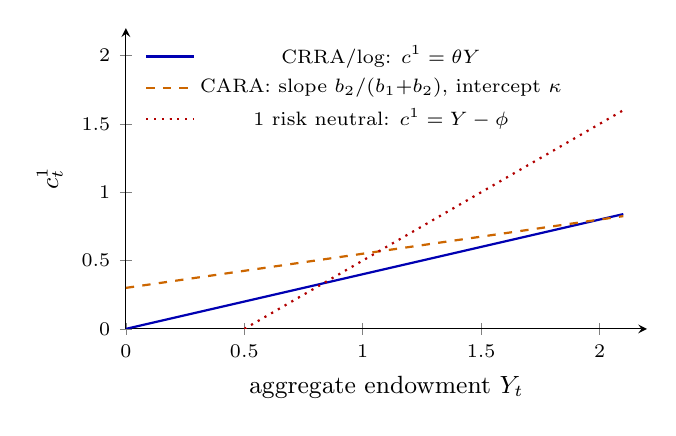
\begin{tikzpicture}
\begin{axis}[width=8.2cm,height=5.4cm,xmin=0,xmax=2.2,ymin=0,ymax=2.2,
  axis lines=left,xlabel={aggregate endowment $Y_t$},ylabel={$c^1_t$},
  xlabel style={font=\small},ylabel style={font=\small},tick label style={font=\scriptsize},
  legend style={font=\scriptsize,at={(0.02,0.98)},anchor=north west,draw=none,fill=none}]
  \addplot[blue!70!black,thick,domain=0:2.1]{0.4*x};
  \addlegendentry{CRRA/log: $c^1=\theta Y$}
  \addplot[orange!80!black,thick,dashed,domain=0:2.1]{0.25*x+0.3};
  \addlegendentry{CARA: slope $b_2/(b_1{+}b_2)$, intercept $\kappa$}
  \addplot[red!70!black,thick,dotted,domain=0.5:2.1]{x-0.5};
  \addlegendentry{1 risk neutral: $c^1=Y-\phi$}
\end{axis}
\end{tikzpicture}
\end{center}
\emph{How to read the figure.} The horizontal axis is aggregate endowment $Y_t$, the vertical axis is household 1's consumption. The slope of each line is the share of aggregate risk household 1 bears. With log/CRRA preferences it bears a constant proportion (ray through the origin); with CARA a constant slope plus a fixed transfer; if household 1 is risk neutral the slope is 1 and household 2's consumption $Y_t-c^1_t=\phi$ is flat.

\begin{tipbox}
CRRA (log) $\Rightarrow$ constant consumption \emph{shares}; CARA $\Rightarrow$ constant \emph{slopes} plus a transfer; a risk-neutral agent fully insures the risk-averse one. In every case only aggregate risk is shared --- idiosyncratic risk is fully diversified away under complete markets.
\end{tipbox}

%======================================================================
\subsection{Pricing redundant assets; the risk-neutral measure \pg{26}}

\paragraph{Setup.} Two dates as in the two-state example. States $s$ at date 1 occur with physical probabilities $\pi(s)$; AD prices $q(s)$ are known. A \emph{redundant asset} is any asset whose payoff $x(s)$ (in each state $s$) can be replicated by a portfolio of AD securities: hold $x(s)$ units of the AD security for state $s$.

\paragraph{No arbitrage.} Two portfolios with identical payoffs in every state must have the same price; otherwise one could buy the cheap one, sell the expensive one, and earn a riskless profit. Hence:
\begin{align*}
  P(x) &= \sum_s q(s)\,x(s) && \text{(cost of the replicating AD portfolio)}\\
  &= \sum_s \pi(s)\,\frac{q(s)}{\pi(s)}\,x(s) && \text{(multiply and divide by $\pi(s)$)}\\
  &= E\big[m\,x\big],\qquad m(s)\equiv\frac{q(s)}{\pi(s)}. && \text{(definition of expectation)}
\end{align*}
Using $q(s)=\beta\pi(s)u'(c(s))/u'(c_0)$ from the two-state example,
\[
  m(s)=\beta\,\frac{u'(c(s))}{u'(c_0)} = \text{IMRS (intertemporal marginal rate of substitution)}.
\]
$m$ is the stochastic discount factor: it measures how much the household values a payoff in each state. It is the static counterpart of $M_{t,t+1}$ in \eqref{eq:s4_sdf}.

\paragraph{Risk-free rate.} A risk-free bond pays $x(s)=1$ in every state. Its price is
\[
  \sum_sq(s)=\sum_s\pi(s)m(s)=E[m]\equiv\frac{1}{R_f}
  \quad\Longrightarrow\quad R_f=\frac{1}{E[m]} \quad\text{(HW3 Q2(c))}.
\]
The gross risk-free rate is the inverse of the expected IMRS.

\paragraph{Risk-neutral (equivalent martingale) measure.} Define
\[
  \pi^*(s)\equiv R_f\,q(s) = R_f\,\pi(s)\,m(s) = \frac{m(s)}{E[m]}\,\pi(s).
\]
Each $\pi^*(s)>0$ (since $q(s)>0$), and they sum to one:
$\sum_s\pi^*(s)=R_f\sum_sq(s)=R_f\cdot\frac{1}{R_f}=1$. So $\pi^*$ is a probability measure: the physical probabilities reweighted by $m(s)/E[m]$. Now rewrite the pricing formula:
\begin{align*}
  P(x) &= \sum_s q(s)\,x(s) = \sum_s \frac{\pi^*(s)}{R_f}\,x(s) && \text{(since $q(s)=\pi^*(s)/R_f$)}\\
       &= \frac{1}{R_f}\,E^*[x], && \text{($E^*$: expectation under $\pi^*$)}
\end{align*}
\begin{keybox}[title=Risk-neutral pricing]
\[
  P(x) = E[m\,x] = \frac{E^*[x]}{R_f},\qquad \pi^*(s)=\frac{m(s)}{E[m]}\,\pi(s).
\]
\begin{itemize}
  \item Risk-averse agents: $m(s)$ is high in bad states (low $c(s)$, high $u'$), so $\pi^*$ \emph{overweights bad states} and \emph{underweights good states}.
  \item Risk-neutral agents: $u'$ constant, so $m(s)=\beta$ for all $s$, $m(s)/E[m]=\beta/\beta=1$, and $\pi^*(s)=\pi(s)$. Prices are then simply discounted expected payoffs.
\end{itemize}
\end{keybox}
Interpretation: all risk adjustment can be put either into the discount factor ($E[mx]$ with physical probabilities) or into the probabilities ($E^*[x]/R_f$ with a risk-free discount rate). Both give the same price.

\paragraph{Numerical example.} Let $\pi(1)=\pi(2)=\tfrac12$, $\beta=0.95$, log utility, $c_0=1$, $c(1)=1.1$ (good state), $c(2)=0.9$ (bad state).
\begin{itemize}
  \item SDF: $m(1)=0.95/1.1\approx0.864$, \ $m(2)=0.95/0.9\approx1.056$; \ $E[m]\approx0.960$, so $R_f\approx1.042$.
  \item Risk-neutral probabilities: $\pi^*(s)=m(s)/(2E[m])$, giving $\pi^*(1)=\frac{1/1.1}{1/1.1+1/0.9}=0.45$ and $\pi^*(2)=0.55$. The bad state gets more weight than its physical probability $0.5$.
  \item Claim to consumption, $x(s)=c(s)$: $P=E[mx]=\tfrac12(0.95)+\tfrac12(0.95)=0.95$. Check: $E^*[x]/R_f=(0.45\cdot1.1+0.55\cdot0.9)/1.042=0.99/1.042\approx0.95$.
  \item Its expected return is $E[x]/P=1/0.95\approx1.053>R_f\approx1.042$: the asset pays off in good times, so it carries a risk premium.
\end{itemize}
